\documentclass{beamer}

\usepackage{natbib}

\usepackage[frenchb]{babel}

\usepackage[T1]{fontenc}

\usepackage[utf8]{inputenc}

\usepackage{amsmath}

\usepackage{tcolorbox}

\usepackage{lipsum}

\usepackage[labelformat=empty]{caption}

\usepackage{cclicenses}

\usetheme{Darmstadt}

\title{Hygiène cryptographique}

\author{\cc Ilan 'trog' Dubois}

\AtBeginSection[]
{
    \begin{frame}
        \frametitle{Sommaire}
            \tableofcontents[currentsection]
    \end{frame}
}

\begin{document}
    \begin{frame}
        \titlepage
    \end{frame}
    \section{Mb dszquphsbqijf}
    \subsection{Définitions}
        \begin{frame}{label=vocabulaire}
            \frametitle{Vocabulaire}
            \begin{center}
                \begin{itemize}
                    \item \textbf{Chiffrer}: Rendre incompréhensible un messgae pour qui n'aurait pas la clé.
                    \item \textbf{Déchiffrer}: Rendre à un message sa forme originale à l'aide de la clé.
                    \item \textbf{Décrypter}: Rendre à un message sa forme originale sans utiliser de clé (casser le code).
                    \begin{tcolorbox}[colback=green!5,colframe=green!40!black,title=Mais crypter alors ?]
                      En anglais chiffrer se dit \textit{encrypt}, d'où la confusion courante avec le terme \textit{crypter} qui en français signifie mettre dans une crypte.
                    \end{tcolorbox}
                \end{itemize}
            \end{center}
        \end{frame}
        \begin{frame}{label=utilisation}
            \frametitle{Les cas d'utilisation}
            \begin{center}
                \begin{itemize}
                    \item Rendre incompréhensible un document quelconque pour toute personne n'ayant pas la clé.
                    \item Assurer l'intégrité d'un document.
                    \item Assurer l'authenticité d'un document.
                \end{itemize}
            \end{center}
        \end{frame}
    \subsection{Deux principaux types de cryptographie}
        \begin{frame}{label=symmetric}
            \frametitle{La cryptographie symmétrique}
            \begin{center}
                \begin{itemize}
                    \item Chiffrement et déchiffrement se font avec une même clé.
                    \item César, Vigenaire, AES...
                    \item Est très rapide, utilisé pour chiffrer son disque, sa connexion...
                \end{itemize}
            \end{center}
        \end{frame}
        \begin{frame}{label=asymmetric}
            \frametitle{La cryptographie asymmétrique}
            \begin{center}
                \begin{itemize}
                    \item Utilise une paire de clé \textit{public}/\textit{privé}.
                    \item Le chiffrement se fait avec une clé publique. Le déchiffrement nécessite la clé privée.
                    \item DSA, RSA, Ed25519...
                    \item Plus lent mais aussi très pratique dans le cas où les parties ne partagent pas encore de \textit{secret}. Sert ainsi souvent à initier une connexion avec un chiffrement symmétrique. Votre clé SSH est basé sur ce type de cryptographie.
                \end{itemize}
            \end{center}
        \end{frame}
        \begin{frame}
            \begin{center}
                \begin{figure}
                    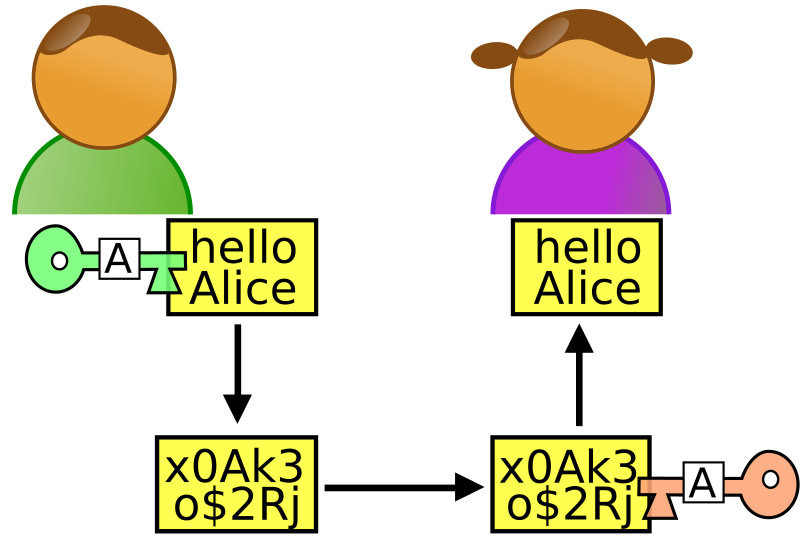
\includegraphics[scale=0.30]{img/asymmetric.png}
                    \caption{\cc --- odder}
                \end{figure}
            \end{center}
        \end{frame}
    \subsection{Bien choisir les paramètres}
        \begin{frame}{label=fails}
            \frametitle{Epic fail}
            \begin{center}
                \begin{figure}
                    
\includegraphics[scale=0.15]{img/plain.jpg}
                    \caption{Image originale}
                \end{figure}
                \pause
                \begin{figure}
                    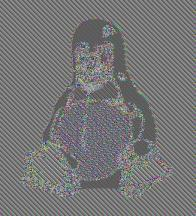
\includegraphics[scale=0.15]{img/aes_no_chain.jpg}
                    \caption{Chiffré sans chaînage}
                \end{figure}
                \pause
                \begin{figure}
                    
\includegraphics[scale=0.15]{img/aes_chain.jpg}
                    \caption{Chiffré avec chaînage}
                \end{figure}
                \cc --- Papa November \& Dr Juzam
            \end{center}
        \end{frame}
    \section{PGP}
    \subsection{Présentation}
        \begin{frame}{label=history}
            \frametitle{Un petit historique}
            \begin{center}
                \begin{itemize}
                    \item Protocole inventé en 1991 par Phil Zimmerman, également inventeur de ZRTP. Destiné au début pour les emails.
                    \item Sa grande performance et sécurité ont fait que PGP est utilisé pour bien d'autres objectifs aujourd'hui, aptitude utilise GPG pour signer les paquets, Debian l'utilise pour son système de vote relative aux orientations de développement.
                    \item L'implémentation la plus connue est GPG (GNU Privacy Guard). Elle est maintenue par un petit groupe de dev berlinois, financé depuis peu entre autre par Facebook.
                    \item Phil Zimmerman était poursuivi pour export illégal de munition car la distribution à l'étranger de système de cryptographie utilisant des clés de plus de 40 bits.
                    \item Pour contourner cette régulation il publia un livre contenant l'intégrlaité du code source de PGP, l'export de livre étant protégé par la constitution américaine. GG
                \end{itemize}
            \end{center}
        \end{frame}
        \begin{frame}{label=utility}
            \frametitle{Utilisation}
            \begin{center}
                \begin{itemize}
                    \item Chiffrer ses communications pour un destinataire \textbf{sans} partage de secret préalable nécessaire.
                    \item \textbf{Authentifier} et assurer l'intégrité des messages par le système de signature.
                    \item Créer un système de confiance \textit{Web of Trust} décentralisé, pas besoin de signature d'une autorité externe.
                    \item Git supporte très bien l'utilisation de GPG, je vous recommande de signer au moins vos tags, ce qui permettra d'authentifier les versions qui seront utilisées.
                \end{itemize}
                \begin{tcolorbox}[colback=green!5,colframe=green!40!black,title=Pourquoi authentifier ?]
                    La signature permet d'authentifier l'origin d'un fichier. On peut donc s'assurer qu'un build, une release ou autre n'a pas été modifié.
                    Dans le cas d'un programme, on s'assure alors qu'aucune back door n'a été ajoutée par exemple ;)
                \end{tcolorbox}
            \end{center}
        \end{frame}
        \appendix
        \begin{frame}
            \bibliography{src/crypto}{}
            \bibliographystyle{plain}
        \end{frame}
\end{document}
